% В этом файле следует писать текст работы, разбивая его на
% разделы (section), подразделы (subsection) и, если нужно,
% главы (chapter).

% Предварительно следует указать необходимую информацию
% в файле SETUP.tex

%% В этот файл не предполагается вносить изменения

% В этом файле следует указать информацию о себе
% и выполняемой работе.

\documentclass [fontsize=14pt, paper=a4, pagesize, DIV=calc]%
{scrartcl}
% ВНИМАНИЕ! Для использования глав поменять
% scrartcl на scrreprt

% Здесь ничего не менять
\usepackage [T2A] {fontenc}   % Кириллица в PDF файле
\usepackage [utf8] {inputenc} % Кодировка текста: utf-8
\usepackage [russian] {babel} % Переносы, лигатуры

%%%%%%%%%%%%%%%%%%%%%%%%%%%%%%%%%%%%%%%%%%%%%%%%%%%%%%%%%%%%%%%%%%%%%%%%
% Создание макроса управления элементами, специфичными
% для вида работы (курс., бак., маг.)
% Здесь ничего не менять:
\usepackage{ifthen}
\newcounter{worktype}
\newcommand{\typeOfWork}[1]
{
	\setcounter{worktype}{#1}
}

% ВНИМАНИЕ!
% Укажите тип работы: 0 - курсовая, 1 - бак., 2 - маг.,
% 3 - бакалаврская с главами.
\typeOfWork{1}
% Считается, что курсовая и бак. бьются на разделы (section) и
% подразделы (subsection), а маг. — на главы (chapter), разделы и
%  подразделы. Если хочется,
% чтобы бак. была с главами (например, если она большая),
% надо выбрать опцию 3.

% Если при выборе 2 или 3 вы забудете поменять класс
% документа на scrreprt (см. выше, в самом начале),
% то получите ошибку:
% ./aux/appearance.tex:52: Package scrbase Error: unknown option ` chapterprefix=

%%%%%%%%%%%%%%%%%%%%%%%%%%%%%%%%%%%%%%%%%%%%%%%%%%%%%%%%%%%%%%%%%%%%%%%%
% Информация об авторе и работе для титульной страницы

\usepackage {titling}

% Имя автора в именительном падеже (для маг.)
\newcommand {\me}{%
И.\,И.~Иванов%
}

% Имя автора в родительном падеже (для курсовой и бак.)
\newcommand {\byme}{%
С.\,Е.~Дегтярева%
}

% Научный руководитель
\newcommand{\supervisor}%
{ассистент Н. Н. Ячменева}

% идентифицируем пол (только для курсовой и бак.)
\newcommand{\bystudent}{
Студентки %Студентки % Для курсовой: с большой буквы
}

% Год публикации
\date{2017}

% Название работы
\title{Машинное обучение в задаче распознавания хронических заболеваний почек на основе медицинских показателей}

% Кафедра
%

\newcommand {\direction} {%
Направление подготовки\\02.\ifthenelse{\value{worktype} = 2}{04}{03}.02 ---
Фундаментальная информатика\\и информационные технологии%
}

%%%%%%%%%%%%%%%%%%%%%%%%%%%%%%%%%%%%%%%%%%%%%%%%%%%%%%%%%%%%%%%%%%%%%%%%
% Другие настраиваемые элементы текста

% Листинги с исходным кодом программ: укажите язык программирования
\usepackage{listings}
\lstset{
    language=[ISO]C++,%  Язык указать здесь
    basicstyle=\small\ttfamily,
    breaklines=true,%
    showstringspaces=false%
    inputencoding=utf8x%
}
% полный список языков, поддерживаемых данным пакетом, есть,
% например, здесь (стр. 13):
% ftp://ftp.tex.ac.uk/tex-archive/macros/latex/contrib/listings/listings.pdf

% Нумерация списков: можно при необходимести
% изменять вид нумерации (например, добавлять правую скобку).
% По умолчанию буду списки вида:
% 1.
% 2.
% Изменять вид нумерации можно в начале нумерации:
% \begin{enumerate}[1)] (В квадратных скобках указан желаемый вид)
\usepackage[shortlabels]{enumitem}
                    \setlist[enumerate, 1]{1.}

% Гиперссылки: настройте внешний вид ссылок
\usepackage%
[pdftex,unicode,pdfborder={0 0 0},draft=false,%backref=page,
    hidelinks, % убрать, если хочется видеть ссылки: это
               % удобно в PDF файле, но не должно появиться на печати
    bookmarks=true,bookmarksnumbered=false,bookmarksopen=false]%
{hyperref}


\usepackage {amsmath}      % Больше математики
\usepackage {amssymb}
\usepackage {textcase}     % Преобразование к верхнему регистру
\usepackage {indentfirst}  % Красная строка первого абзаца в разделе

\usepackage {fancyvrb}     % Листинги: определяем своё окружение Verb
\DefineVerbatimEnvironment% с уменьшенным шрифтом
	{Verb}{Verbatim}
	{fontsize=\small}

% Вставка рисунков
\usepackage {graphicx}

% Общее оформление
% ----------------------------------------------------------------
% Настройка внешнего вида

%%% Шрифты

% если закомментировать всё — консервативная гарнитура Computer Modern
\usepackage{paratype} % профессиональные свободные шрифты
%\usepackage {droid}  % неплохие свободные шрифты от Google
%\usepackage{mathptmx}
%\usepackage {mmasym}
%\usepackage {psfonts}
%\usepackage{lmodern}
%var1: lh additions for bold concrete fonts
%\usepackage{lh-t2axccr}
%var2: the package below could be covered with fd-files
%\usepackage{lh-t2accr}
%\usepackage {pscyr}

% Геометрия текста

\usepackage{setspace}       % Межстрочный интервал
\onehalfspacing

\newlength\MyIndent
\setlength\MyIndent{1.25cm}
\setlength{\parindent}{\MyIndent} % Абзацный отступ
\frenchspacing            % Отключение лишних отступов после точек
\KOMAoptions{%
    DIV=calc,         % Пересчёт геометрии
    numbers=endperiod % точки после номеров разделов
}

                            % Консервативный вариант:
%\usepackage                % ручное задание геометрии
%[%                         % (не рекомендуется в проф. типографии)
%  margin = 2.5cm,
  %includefoot,
  %footskip = 1cm
%] %
%  {geometry}

%%% Заголовки


\ifthenelse{{\value{worktype} > 1}}{%
  \KOMAoptions{%
      headings=normal,   % размеры заголовков поменьше стандартных
      chapterprefix=true,% Печатать слово Глава
      appendixprefix=true% Печатать слово Приложение
  }
}{% Печатать слово Приложение даже если нет глав
  \newcommand*{\appendixmore}{%
    \renewcommand*{\sectionformat}{%
    \appendixname~\thesection\autodot\enskip}
    \renewcommand*{\sectionmarkformat}{%
      \appendixname~\thesection\autodot\enskip}
  }
}

% шрифт для оформления глав и названия содержания
\newcommand{\SuperFont}{\Large\sffamily\bfseries}

% Заголовок главы
\ifthenelse{\value{worktype} > 1}{%
\renewcommand{\SuperFont}{\Large\normalfont\sffamily}
\newcommand{\CentSuperFont}{\centering\SuperFont}
\usepackage{fncychap}
\ChNameVar{\SuperFont}
\ChNumVar{\CentSuperFont}
\ChTitleVar{\CentSuperFont}
\ChNameUpperCase
\ChTitleUpperCase
}

% Заголовок (под)раздела с абзацного отступа
\addtokomafont{sectioning}{\hspace{\MyIndent}}

\renewcommand*{\captionformat}{~---~}
\renewcommand*{\figureformat}{Рисунок~\thefigure}

% Плавающие листинги
\usepackage{float}
\floatstyle{ruled}
\floatname{ListingEnv}{Листинг}
\newfloat{ListingEnv}{htbp}{lol}[section]

% точка после номера листинга
\makeatletter
\renewcommand\floatc@ruled[2]{{\@fs@cfont #1.} #2\par}
\makeatother


%%% Оглавление
\usepackage{tocloft}

% шрифт и положение заголовка
\ifthenelse{\value{worktype} > 1}{%
\renewcommand{\cfttoctitlefont}{\hfil\SuperFont\MakeUppercase}
}{
\renewcommand{\cfttoctitlefont}{\hfil\SuperFont}
}

% слово Глава
\usepackage{calc}
\ifthenelse{\value{worktype} > 1}{%
\renewcommand{\cftchappresnum}{Глава }
\addtolength{\cftchapnumwidth}{\widthof{Глава }}
}

% Очищаем оформление названий старших элементов в оглавлении
\ifthenelse{\value{worktype} > 1}{%
\renewcommand{\cftchapfont}{}
\renewcommand{\cftchappagefont}{}
}{
\renewcommand{\cftsecfont}{}
\renewcommand{\cftsecpagefont}{}
}

% Точки после верхних элементов оглавления
\renewcommand{\cftsecdotsep}{\cftdotsep}
%\newcommand{\cftchapdotsep}{\cftdotsep}

\ifthenelse{\value{worktype} > 1}{%
    \renewcommand{\cftchapaftersnum}{.}
}{}
\renewcommand{\cftsecaftersnum}{.}
\renewcommand{\cftsubsecaftersnum}{.}
\renewcommand{\cftsubsubsecaftersnum}{.}

%%% Списки (enumitem)

\usepackage {enumitem}      % Списки с настройкой отступов
\setlist %
{ %
  leftmargin = \parindent, itemsep=.5ex, topsep=.4ex
} %

% По ГОСТу нумерация должны быть буквами: а, б...
%\makeatletter
%    \AddEnumerateCounter{\asbuk}{\@asbuk}{м)}
%\makeatother
%\renewcommand{\labelenumi}{\asbuk{enumi})}
%\renewcommand{\labelenumii}{\arabic{enumii})}

%%% Таблицы: выбрать более подходящие

\usepackage{booktabs} % считаются наиболее профессионально выполненными
%\usepackage{ltablex}
%\newcolumntype {L} {>{---}l}

%%% Библиография

\usepackage{csquotes}        % Оформление списка литературы
\usepackage[
  backend=biber,
  hyperref=auto,
  sorting=none, % сортировка в порядке встречаемости ссылок
  language=auto,
  citestyle=gost-numeric,
  bibstyle=gost-numeric
]{biblatex}
\addbibresource{biblio.bib} % Файл с лит.источниками

% Настройка величины отступа в списке
\ifthenelse{\value{worktype} < 2}{%
\defbibenvironment{bibliography}
  {\list
     {\printtext[labelnumberwidth]{%
    \printfield{prefixnumber}%
    \printfield{labelnumber}}}
     {\setlength{\labelwidth}{\labelnumberwidth}%
      \setlength{\leftmargin}{\labelwidth}%
      \setlength{\labelsep}{\dimexpr\MyIndent-\labelwidth\relax}% <----- default is \biblabelsep
      \addtolength{\leftmargin}{\labelsep}%
      \setlength{\itemsep}{\bibitemsep}%
      \setlength{\parsep}{\bibparsep}}%
      \renewcommand*{\makelabel}[1]{\hss##1}}
  {\endlist}
  {\item}
}{}

% ----------------------------------------------------------------
% Настройка переносов и разрывов страниц

\binoppenalty = 10000      % Запрет переносов строк в формулах
\relpenalty = 10000        %

\sloppy                    % Не выходить за границы бокса
%\tolerance = 400          % или более точно
\clubpenalty = 10000       % Запрет разрывов страниц после первой
\widowpenalty = 10000      % и перед предпоследней строкой абзаца

% ----------------------------


% Стили для окружений типа Определение, Теорема...
% Оформление теорем (ntheorem)

\usepackage [thmmarks, amsmath] {ntheorem}
\theorempreskipamount 0.6cm

\theoremstyle {plain} %
\theoremheaderfont {\normalfont \bfseries} %
\theorembodyfont {\slshape} %
\theoremsymbol {\ensuremath {_\Box}} %
\theoremseparator {:} %
\newtheorem {mystatement} {Утверждение} [section] %
\newtheorem {mylemma} {Лемма} [section] %
\newtheorem {mycorollary} {Следствие} [section] %

\theoremstyle {nonumberplain} %
\theoremseparator {.} %
\theoremsymbol {\ensuremath {_\diamondsuit}} %
\newtheorem {mydefinition} {Определение} %

\theoremstyle {plain} %
\theoremheaderfont {\normalfont \bfseries} 
\theorembodyfont {\normalfont} 
%\theoremsymbol {\ensuremath {_\Box}} %
\theoremseparator {.} %
\newtheorem {mytask} {Задача} [section]%
\renewcommand{\themytask}{\arabic{mytask}}

\theoremheaderfont {\scshape} %
\theorembodyfont {\upshape} %
\theoremstyle {nonumberplain} %
\theoremseparator {} %
\theoremsymbol {\rule {1ex} {1ex}} %
\newtheorem {myproof} {Доказательство} %

\theorembodyfont {\upshape} %
%\theoremindent 0.5cm
\theoremstyle {nonumberbreak} \theoremseparator {\\} %
\theoremsymbol {\ensuremath {\ast}} %
\newtheorem {myexample} {Пример} %
\newtheorem {myexamples} {Примеры} %

\theoremheaderfont {\itshape} %
\theorembodyfont {\upshape} %
\theoremstyle {nonumberplain} %
\theoremseparator {:} %
\theoremsymbol {\ensuremath {_\triangle}} %
\newtheorem {myremark} {Замечание} %
\theoremstyle {nonumberbreak} %
\newtheorem {myremarks} {Замечания} %


% Титульный лист
% Макросы настройки титульной страницы
% В этот файл не предполагается вносить изменения

%\usepackage {showframe}

% Вертикальные отступы на титульной странице
\newcommand{\vgap}{\vspace{16pt}}

% Помещение города и даты в нижний колонтитул
\usepackage{scrlayer}
\DeclareNewLayer[
  foot,
  foreground,
  contents={%
    \raisebox{\dp\strutbox}[\layerheight][0pt]{%
      \parbox[b]{\layerwidth}{\centering Ростов-на-Дону\\ \thedate%
       \\\mbox{}
       }}%
  }
]{titlepage.foot.fg}
\DeclareNewPageStyleByLayers{titlepage}{titlepage.foot.fg}


\AtBeginDocument %
{ %
  %
  \begin{titlepage}
  %
    \thispagestyle{titlepage}

    {\centering
    %
    \MakeTextUppercase {МИНИСТЕРСТВО ОБРАЗОВАНИЯ И НАУКИ РФ}

    \vgap

    Федеральное государственное автономное образовательное\\
    учреждение высшего образования\\
    \MakeTextUppercase {Южный федеральный университет}

    \vgap

	Институт математики, механики и компьютерных наук
    имени~И.\,И.\,Воровича

    \vgap

    \direction

    \vspace* {\fill}

    \ifthenelse{\value{worktype} = 2}{%
    \me

    \vgap}{}

    {\usefont{T2A}{PTSansCaption-TLF}{m}{n}
    \MakeTextUppercase{\thetitle}}

    \ifthenelse{\value{worktype} = 2}{%
     \vgap

    Магистерская диссертация}{}
    \ifthenelse{\value{worktype} = 0}{
     \vgap

    Курсовая работа
    }{}%
    \ifthenelse{\value{worktype} = 1 \OR \value{worktype} = 3}{
     \vgap

    Выпускная квалификационная работа\\
    на степень бакалавра
    }{}%

    \vspace {\fill}

    \begin{flushright}
    \ifthenelse{\value{worktype} = 0 \OR 
                \value{worktype} = 1 \OR
                \value{worktype} = 3}{
      \bystudent \ifthenelse{\value{worktype} = 0}{3}{4}\ курса\\
      \byme
    }{}

    \vgap

    Научный руководитель:\\
    \supervisor\\
    \ifthenelse{\value{worktype} = 2}{%
    Рецензент:\\
    ученая степень, ученое звание, должность
    И. О. Фамилия
    }{}
	\end{flushright}
\ifthenelse{\value{worktype} = 0}{
\vspace{\fill}
        \begin{flushleft}
          \begin{tabular}{cc}
            \underline{\hspace{4cm}}&\underline{\hspace{5cm}}\\
            {\small оценка (рейтинг)} & {\small  подпись руководителя}\\
          \end{tabular}
          \\[1cm]
        \end{flushleft}
}{}
\ifthenelse{\value{worktype} = 1 \OR \value{worktype} = 3}{
\vspace{\fill}
        \begin{flushleft}
Допущено к защите:\\руководитель направления ФИИТ
\underline{\hspace{4cm}}
В.\,С.\,Пилиди
        \end{flushleft}
}{}


  	\vspace {\fill}
  %Ростов-на-Дону

    %\thedate

  }\end{titlepage}
  %
  %
  \tableofcontents
  %
  \clearpage
} %


% Команды для использования в тексте работы


% макросы для начала введения и заключения
\newcommand{\Intro}{\addsec{Введение}}
\ifthenelse{\value{worktype} > 1}{%
    \renewcommand{\Intro}{\addchap{Введение}}%
}

\newcommand{\Conc}{\addsec{Заключение}}
\ifthenelse{\value{worktype} > 1}{%
    \renewcommand{\Conc}{\addchap{Заключение}}%
}

% Правильные значки для нестрогих неравенств и пустого множества
\renewcommand {\le} {\leqslant}
\renewcommand {\ge} {\geqslant}
\renewcommand {\emptyset} {\varnothing}

% N ажурное: натуральные числа
\newcommand {\N} {\ensuremath{\mathbb N}}

% значок С++ — используйте команду \cpp
\newcommand{\cpp}{%
C\nolinebreak\hspace{-.05em}%
\raisebox{.2ex}{+}\nolinebreak\hspace{-.10em}%
\raisebox{.2ex}{+}%
}

% Неразрывный дефис, который допускает перенос внутри слов,
% типа жёлто-синий: нужно писать жёлто"/синий.
\makeatletter
    \defineshorthand[russian]{"/}{\mbox{-}\bbl@allowhyphens}
\makeatother


\endinput

% Конец файла



\NewBibliographyString{langjapanese}
\NewBibliographyString{fromjapanese}

\begin{document}

\Intro

В наши дни машинное обучение приобретает все большую актуальность в виду роста количества населения, благ, произведенных человеком и активного внедрения информационных технологий во множество сфер жизни. Так, одной из областей применения является медицина. Например, задача постановления диагноза хронического заболевания, имеющего определенные симптомы, может быть решена методами машинного обучения, ведь искусственный интеллект способен анализировать данные почти также, как это делает человек. Решение данной задачи позволило бы сократить время, затрачиваемое врачами на диагностику заболевания.

В рамках данной работы в качестве метода машинного обучения были выбраны нейронные сети, а именно многослойный персептрон с обратным распространением ошибки и самоорганизующаяся карта Кохонена. Данные алгоритмы будут продемонстрированы на задаче распознавания хронического заболевания почек.

\newpage

\section{Постановка задачи}
Целью работы является построение нейронных сетей, способных распознавать хронические заболевания почек с максимальной точностью.

Выделим следующие задачи:

\begin{enumerate}
	\item
		Обработка и нормализация исходных данных.
	\item 
		Реализация многослойного персептрона и алгоритма обратного распространения ошибки.
	\item 
		Получение результатов работы с учетом изменения точности, скорости обучения и размера обучающей выборки. 
	\item 
		Анализ полученных данных.
	\item
		Установление влияния конкретных атрибутов на работу сети.
	\item 
		Сравнение результатов работы нейронной сети и библиотечного аналога.
	\item
		Реализация самоорганизующейся карты Кохонена.
	\item
		Анализ работы сети.
	\item
		Сравнение между собой реализованного многослойного персептрона, его библиотечного аналога и самоорганизующейся карты Кохонена.
\end{enumerate}
\newpage

\section{Описание и обработка входных данных}
 В качестве обучающей выборки для нейронной сети была выбрана база данных, содержащая ряд медицинских показателей, непосредственно диагноз и имеющая следующий формат:
 
 \begin{itemize}
 	\item
 		Секция с перечислением атрибутов и областью значений, которые они принимают.
 	\item 
 		Секция с данными.
 \end{itemize}
 
\subsection{Обработка данных}

	Так как нейронные сети принимают на вход исключительно числовые данные, необходима обработка исходной базы.
	
	Таким образом, были изменены следующие атрибуты:
	\\
	\begin{table}[H]
	\centering
	\begin{tabular}{llr}
	\toprule
	Атрибут  & Исходный формат & Результат \\
	\midrule 
	 rbc (red blood cells)      & normal / abnormal    & 1 / 2 \\
	 pc (pus cell)      & normal / abnormal    & 1 / 2 \\
	 pcc (pus cell clumps)      & present / notpresent    & 1 / 2 \\
	 ba (bacteria)      & present / notpresent   & 1 / 2 \\
	 htn (hypertension)      & yes / no   & 1 / 2 \\
	 dm (diabetes mellitus)      & yes / no   & 1 / 2 \\
	 cad (coronary artery disease)      & yes / no   & 1 / 2 \\
	 appet (appetite)      & good / poor   & 1 / 2 \\
	 pe (pedal edema)      & yes / no   & 1 / 2 \\
	 ane (anemia)      & yes / no   & 1 / 2 \\
	 class      & ckd / notckd   & 0 / 1 \\
	 unknown value & ?  & 0 \\

	\bottomrule
	\end{tabular}
	\end{table}

\subsection{Нормализация данных}
Хорошо известно, что большинство методов градиентного спуска являются чувствительными к шкалированию данных. Если игнорировать эту особенность, будет оказываться дополнительное влияние на нейроны, что в итоге приводит к неверным решениям. Поэтому перед использованием данные необходимо нормализовать. 


Для этого будем использовать следующую формулу:
\\
$$ y=\frac{(x - x_{min})(d_2 - d_1)}{x_{max}-x_{min}}+d_1 $$
\\
$x$ \small - значение подлежащее нормализации, \\
\normalsize $x_{min} , x_{max}$ \small - интервал значений  \normalsize $x$ \small, \\
\normalsize $d_1 , d_2$ \small - интервал, к которому будет приведено значение \normalsize $x$ \small ; \\
\\
\normalsize
В нашей задаче интервалом будет $[0,1]$, что приведет формулу к следующему виду:

$$ y=\frac{x - x_{min}}{x_{max}-x_{min}}$$ 

% Если typeOfWork в SETUP.tex задан как 2 или 3, то начинать
% надо не с section (раздел), а с главы (chapter)

\subsection {Пример}
Исходные данные представляют собой набор строк имеющих следующий вид:
\begin{center}
48,80,1.020,1,0,?,normal,notpresent,notpresent,121,
36,1.2,?,?,15.4,44,7800,5.2,yes,yes,no,good,no,no,ckd 
\end{center}
Далее для удобства восприятия будем рассматривать данную строку в виде таблицы, где каждому значению соответсвует одна строка.
\begin{table}[H]
\begin{tabular}{llcc}
\toprule
Значение  & Атрибут  & Обработка & Нормализация \\
\midrule 
48 & age & 48 & 0.5333  \\
80 & bp (blood pressure) & 80 & 0.4444  \\
1.020 & sg (specific gravity) & 1.020 & 0.9951  \\
1 & al (albumin) & 1 & 0.2  \\
0 & su (sugar) & 0 & 0  \\
? & rbc (red blood cells) & 0 & 0  \\
normal & pc (pus cell) & 1 & 0.5 \\
notpresent & pcc (pus cell clumps) & 2 & 1  \\
notpresent & ba (bacteria) & 2 & 1 \\
121 & bgr (blood glucose random) & 121 & 0.2469 \\
36 & bu (blood urea) & 36 & 0.0921  \\
1.2 & sc (serum creatinine) & 1.2 & 0.0158  \\
? & sod (sodium) & 0 &  0 \\
? & pot (potassium) & 0 & 0  \\
15.4 & hemo (hemoglobin) & 15.4 & 0.8652  \\
44 & pcv (packed cell volume) & 44 & 0.8148  \\
7800 & wbcc (white blood cell count) & 7800 & 0.2955  \\
5.2 & rbcc (red blood cell count) & 5.2 & 0.65  \\
yes & htn (hypertension) & 1 & 0.5  \\
yes & dm (diabetes mellitus) & 1 & 0.5  \\
no  & cad (coronary artery disease) & 2 & 1  \\
good & appet (appetite) & 1 & 0.5  \\
no & pe (pedal edema) & 2 & 1  \\
no & ane (anemia) & 2 & 1  \\
ckd & class & 0 & 0  \\
\bottomrule
\end{tabular}
\end{table}

\newpage

\section {Многослойный персептрон}
В рамках данной работы в качестве метода машинного обучения были выбраны нейронные сети. Одной из них является многослойный персептрон.
\begin{figure}[H]
\center{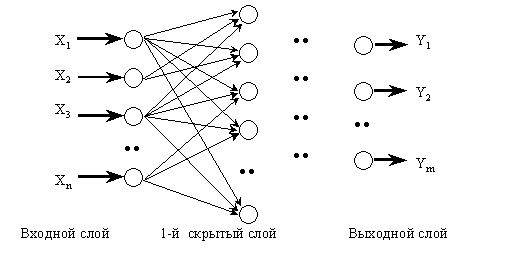
\includegraphics[width=0.7\linewidth]{img/perceptron.png} \\ \footnotesize \textit{ Рис. Архитектура многослойного персептрона}}
\end{figure}
В качестве функции активации выбрана сигмоидальная функция имеющая следующий вид:
$$ f(x)=\frac{1}{1+e^{-x}}.$$
В качестве  обучения был выбран метод обратного распространия ошибки, где  среднеквадратичная ошибка вычисляется по формуле:
$$ E(\{w_{i,j}\})=\frac{1}{2}\sum_{k \in Outputs}(t_k-o_k)^2$$ \small
\normalsize $ w_{i,j} $ \small - вес, стоящий на ребре, соединяющем i-й и j-й узлы;\\
\normalsize $ o_k $ \small - выход k-го узла ($k \in Outputs$);\\
\normalsize $ t_k $ \small - правильные ответы сети ($k \in Outputs$);
\normalsize
\\
\\
А веса корректируются по следующей формуле:
$$ \delta_k=o_k(1-o_k)(t_k-o_k).$$
$$ \delta_j=o_k(1-o_k)\sum_{k \in Outputs} \delta_k w_{j,k}.$$
$$ \Delta w_{i,j}(n)=\eta\delta_jo_i.$$ 
$$ w_{i,j}(n)=w_{i,j}(n-1)+\Delta w_{i,j}(n).$$ 
\\
$ \eta $ \small - скорость обучения сети;
\normalsize

\subsection{Анализ размеров обучающей выборки.}
Рассмотрим график соотношения обучающей и тестовой выборки и его влияние на процент верных ответов. Это позволит нам выбрать оптимальный  размер для дальнейшего анализа работы сети.
\begin{figure}[H]
\center{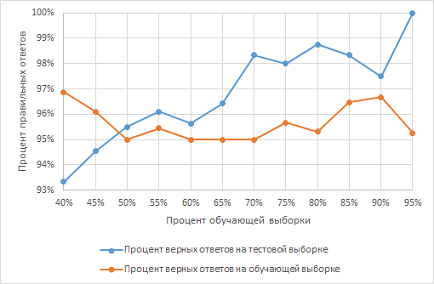
\includegraphics{img/sample.png} \\}
\end{figure}
Исходя из графика можно сделать вывод : чем больше размер обучающей выборки, тем выше количество верных ответов. Однако при чрезмерно большом проценте сеть дает заметно более плохой результат на уже знакомых ей данных. 

\subsection{Анализ параметров.}
Большое влияние на работу сети оказывает правильный подбор параметров. В нашем случае это скорость обучения и точность. Рассмотрим их влияние в виде графика.
\begin{figure}[H]
\center{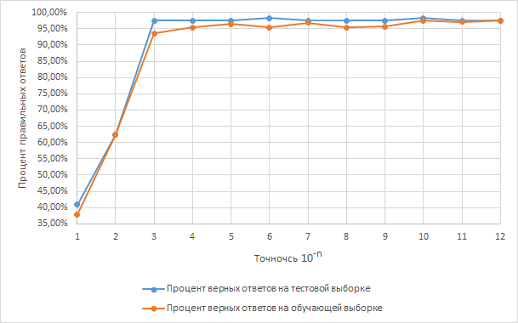
\includegraphics{img/accuracy.png} \\ \footnotesize \textit{ Рис. График влияния точности, при скорости обучения 0.2}}
\end{figure}
Исходя из графика видно, что нет смысла в установлении достаточно высокой точности, так как это не вносит существенных изменений в результат. 
\begin{figure}[H]
\center{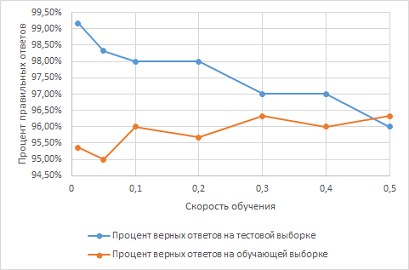
\includegraphics{img/speed.png} \\ \footnotesize \textit{ Рис. График влияния скорости обучения, при точности $10^6$}}
\end{figure}
Исходя из графика делаем вывод : чем меньше скорость обучения, тем выше процент верных ответов сети. Однако, меньшее значение коэффициента соответсвует меньшему шагу коррекции весов. При этом количество итераций, а следовательной и итоговое время обучения сети увеличивается.
\subsection{Сравнение реализованной сети с библиотечным аналогом.}
Для оценки качества работы реализованой сети сравним ее с аналогичной сетью из библиотеки OPENCV при одинаково установленных параметрах.
\begin{figure}[H]
\center{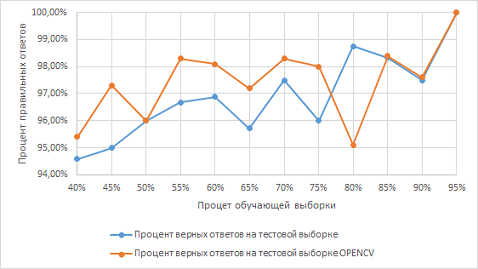
\includegraphics{img/1.png} \\}
\end{figure}
\begin{figure}[H]
\center{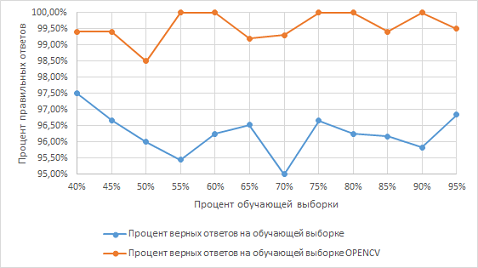
\includegraphics{img/2.png} \\}
\end{figure}
Как видно по графикам, реализованная сеть незначительно уступает библиотеченой по проценту верных ответов на незнакомых данных, но значительно по проценту верных ответов на уже знакомых данных. Однако при этом среднее время затрачиваемое на обучение реализованной сети составляет 0.001 секунды, а для библиотечного аналога 0,987 секунды.
\subsection{Анализ атрибутов.}
Эксперементальным путем было установлено, что не все атрибуты влияют на результат работы сети, что позволило исключить их из списка данных и сократить время затрачиваемое сетью на обучение. Список атрибутов влияющих на результат представлен ниже.
\begin{figure}[H]
\center{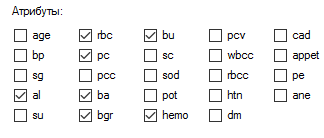
\includegraphics{img/attributes.png} \\}
\end{figure}
\newpage
\section {Самоорганизующаяся карта Кохонена}
В рамках данной работы в качестве метода машинного обучения были выбраны нейронные сети. Одной из них является самоорганизующаяся карта Кохонена.
\begin{figure}[H]
\center{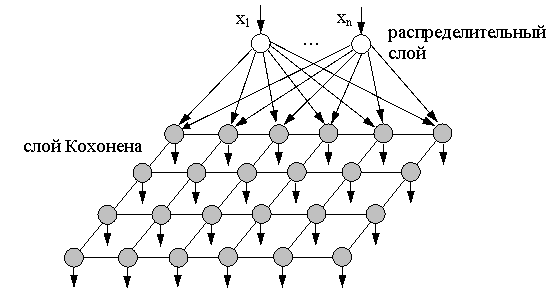
\includegraphics[width=0.8\linewidth]{img/kohonen.png} \\ \footnotesize \textit{ Рис. Архитектура самоорганизующейся карты Кохонена}}
\end{figure}
Победивший нейрон определяется по формуле:
$$ i(x)=\min_j||x-w_j||, j=1,2,..l $$
$l$-\small общее количество нейронов в решетке 
\normalsize
\\
Векторы синаптических весов всех нейронов корректируются следующим образом:
$$w_j(n+1)=w_j(n)+\eta(n)h_{j,i(x)}(n))(x-w_j(n))$$
$\eta(n)$-\small параметр скорости обучения, \normalsize \\ 
$h_{j,i(x)}(n)$-\small функция окрестности с центром в победившем нейроне i(x). \normalsize \\ 
Функция окрестности :
$$ h_{j,i(x)}= exp(-\frac{d^2_{j,i}}{2\sigma^2}).$$
$d_{j,i}$-\small литеральное расстояние между победившим (i) и вторично возбужденным (j) нейронами, \normalsize \\ 
$\sigma$ - \small эффективная ширина топологической окрестности.  \\ 
\normalsize
$$d^2_{i,j}=||r_j-r_i||^2$$
$r_j$ - \small позиция возбуждаемого нейрона j, \\ \normalsize
$r_i$ - \small позиция победившего нейрона i. \\ \normalsize
$$ \sigma(n)=\sigma(0)exp(-\frac{n}{\tau}), n=0,1,2...$$ 
$n$ - \small номер итерации, \\ \normalsize
$\tau$ - \small некоторая временная константа, \\ \normalsize
$\sigma(0)$ - \small начальное значение величины \normalsize $\sigma$ \small в алгоритме SOM.\\ \normalsize

\subsection{Анализ параметров.}
Рассмотрим график на котором отражено влияние точности на процент верных ответов, выдаваемых сетью.
\begin{figure}[H]
\center{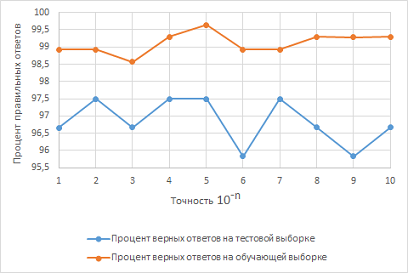
\includegraphics{img/kohonen1.png} \\}
\end{figure}
Исходя из графика видно, что также как и в случае с многослойным персептроном повышение точности не приводит к существенному улучшению результата. Оптимальной будем считать точность $10^4-10^5$.
\subsection{Сравнение с многослойным персептроном.}
А теперь сравним все ранее представленные сети, для того чтобы сделать окончательный выбор об их эффективности для решения поставленной задачи.
\begin{figure}[H]
\center{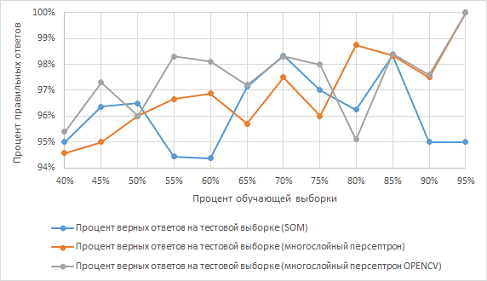
\includegraphics{img/comparison.png} \\}
\end{figure}
\begin{figure}[H]
\center{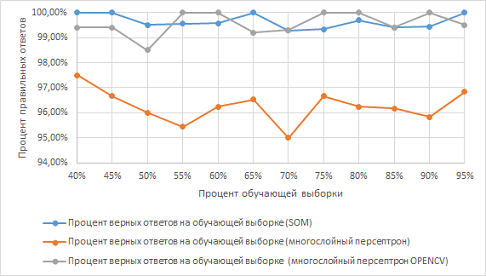
\includegraphics{img/comparison2.png} \\}
\end{figure}
Исходя из графиков можно сделать вывод о том, что самоорганизующаяся карта Кохонена, дает практически такой же результат как и многослойный персептрон, за исключением некоторых соотношений обучающей и тестовой выборки. Однако, карты самоорганизации являются нейронной сетью без учителя, что делает ее более удобной и универсальной в использовании, а также имеющей более простую реализацию по сравнению с персептроном. При этом данная сеть выдает практически такой же результат как и библиотечный классификатор, как на тестовой так и на обучающей выборке, в отличие от реализованного многослойного персептрона, который заметно проигрывает по проценту верных ответов на обучающей выборке своему библиотечному аналогу и самоорганизующейся карте Кохонена.

Также можно сделать вывод о том, что несмотря на незначительную разницу в результатах, которая обусловлена теми или иными особенностями сетей, все они эффективно справляются с поставленой задачей, о чем говорит минимальная отметка процента правильных ответов. 
\newpage 

\Conc
В данном исследовании мы убедились, что машинное обучение позволяет справляться с глобальными задачами, в том числе и в области медицины, выдавая при этом достаточно высокие показатели, сравнимые с резульатом труда человека. 

Существенным плюсом механизма нейронных сетей, является гибкость их применения, а именно, несмотря на то, что в рамках данного исследования их работа была продемонстрирована на конкретной задаче распознавания хронического заболевания почек, все реализованные сети могут использоваться в похожих задачах из сферы медицины и не только. Это может быть, например, установление ряда других заболеваний, по ряду совершенного других медицинских показателей, однако с точки зрения сети, это все равно будет оставаться практически той же самой задачей, которая была рассмотрена в этой работе.

Механизм нейронных сетей уже нашел свое реальное применение в медицине. Ярким примером этого служат сети, способные распознавать рак по фотографиям и отличать злокачественные родинки от доброкачественных. И дальнейшее развитие нейронных сетей в данной области позволит значительно облегчить труд медицинским работникам.\cite{TanAus2013}

\newpage
Помните, что на все пункты списка литературы должны быть ссылки. \LaTeX\ просто не добавит информацию об издании из bib"/файла, если на это издание нет ссылки в тексте. Часто студенты используют в работе  электронные ресурсы: в этом нет ничего зазорного при одном условии: при каждом заимствовании следует ставить соответствующую ссылку. В качестве примера приведём ссылку на сайт нашего института~\autocite{mmcs}.

Для дальнейшего изучения \LaTeX\ рекомендуем книгу Львовского~\autocite{Lvo2003}: она хорошо написана, хотя и несколько устарела.
Обычно стоит искать подсказки на
\href{http://tex.stackexchange.com/}{tex.stackexchange.com}, а также
читать документацию по установленным пакетам с помощью
команды


% Печать списка литературы (библиографии)
\printbibliography[%{}
    heading=bibintoc%
    %,title=Библиография % если хочется это слово
]
% Файл со списком литературы: biblio.bib
% Подробно по оформлению библиографии:
% см. документацию к пакету biblatex-gost
% http://ctan.mirrorcatalogs.com/macros/latex/exptl/biblatex-contrib/biblatex-gost/doc/biblatex-gost.pdf
% и огромное количество примеров там же:
% http://mirror.macomnet.net/pub/CTAN/macros/latex/contrib/biblatex-contrib/biblatex-gost/doc/biblatex-gost-examples.pdf

\appendix
\ifthenelse{\value{worktype} > 1}{%
  \addtocontents{toc}{%
      \protect\renewcommand{\protect\cftchappresnum}{\appendixname\space}%
      \protect\addtolength{\protect\cftchapnumwidth}{\widthof{\appendixname\space{}} - \widthof{Глава }}%
  }%
}{
  \addtocontents{toc}{%
      \protect\renewcommand{\protect\cftsecpresnum}{\appendixname\space}%
      \protect\addtolength{\protect\cftsecnumwidth}{\widthof{\appendixname\space{}}}%
  }%
}

\end{document}
